\section{System Requirements Specification}
\thispagestyle{plain}

\subsection{Purpose}
This is the software requirement specification for the new version of Stedr, both the back-end system that provides content and also the front-end that shows the content and the context of the content to the user. Here the traditional architectural terms back-end - and front-end are used, but there are some subtleties to this term, as the front-end itself is managing a content service of its own. 

\subsection{Intended audience and reading suggestions}
Intended readers for this document are current and future developers, and the customer. The reader should also be noted that the SRS both can be read as a stand-alone document to get an overview of the rationalization behind the development process, but that it also is a part of the project report as a whole


\subsection{References}
The software requirements are based on the standard as provided by ISO/IEC:25010 \cite[10]{25010}, and also the models that can be found in this report's section for architecture and modelling. References to the ISO-standard and other literature are found at the end of the project report under references.

\subsection{Product perspective}
Originally Stedr is a product developed by students at NTNU as a part of the subject TDT4290, and this application will form a basis for out continued development. The state of the existing application is considered to be a working prototype, and to some degrees it is an application that is built up with a traditional server-client architecture. A simple technical overview of the system is provided below. 

\begin{figure}[h!]
\begin{center}
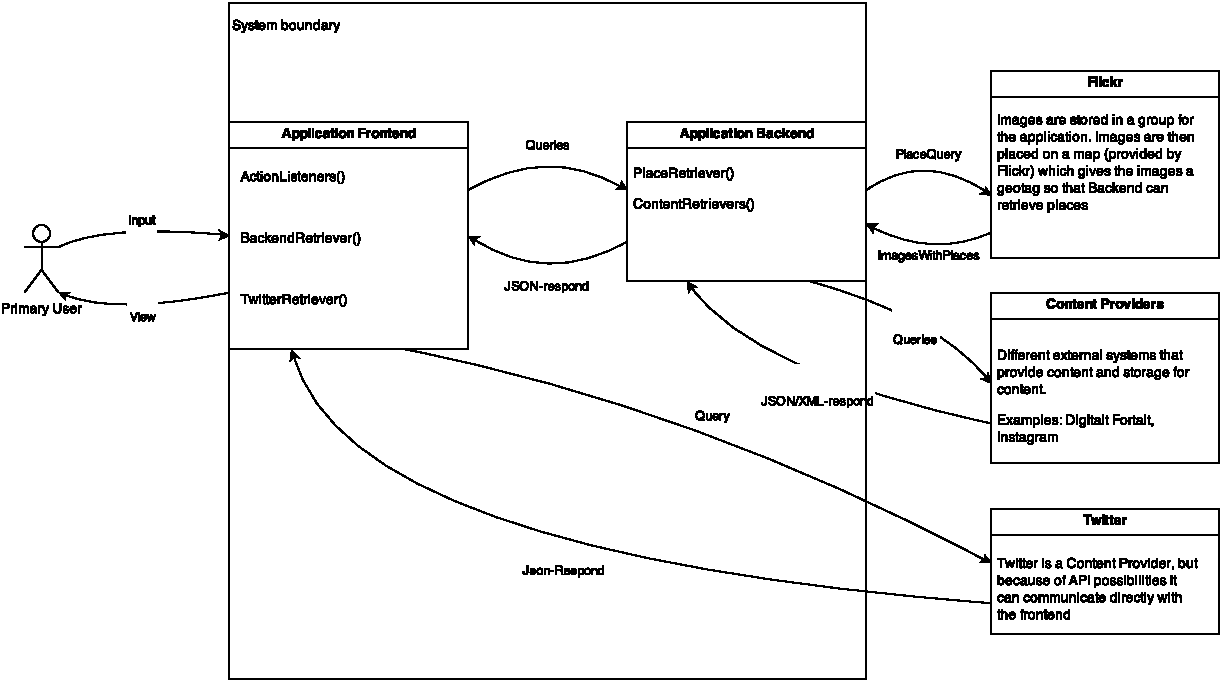
\includegraphics[scale=0.6]{tooverview-architecture}
\caption{A simple technical overview of the architecture}
\end{center}
\end{figure}

\subsection{User classes and characteristics}
The users of the program mainly divide into two categories. One of those groups is the primary user group which are interacting with the smartphone application, front-end, to see content. A typical primary user is an high school student which is introduced to the program in the context of cultural heritage awareness. As mentioned earlier, the broad goal of the application is to make people aware about cultural heritage. If that goal is fulfilled, some primary users of the application will hopefully transit over to become a content provider. 

\noindent

A content provider has the possibility to interact with the system directly, but also he or she can choose to interact with the system more indirectly. This varying degree of interaction will hopefully lower the threshold for users transiting from content consumer to content provider, which is the overall goal of the application. 

\noindent

Another secondary user is the maintainer-administrator. The maintainer-administrator will use a special set of tools to approve creation of the systems places, but these tools are provided by the external system Flickr. Our internal system is communicating with that external system so that applications relevant information is sent from the external to the internal system, but in the end the external system is stand-alone and can not be controlled directly from the internal system. 

\noindent

\subsection{Product functions}

The main features of the program for different user categories are presented as a bullet list below. All of the provided functions by the system are available to every user without the need of registration or approval by the systems maintainer-administrator with one exception relating to adding new places. In addition the user may need to register on external systems to make use of those features.

\noindent


\begin{description}
\item [\textbf{Primary user}]
\end{description}
\begin{itemize}
\item See places on a world map
\item Navigate the map
\item Select places on the map, and look at stories to the related place. 
\item Select places on the map, and look at pictures to the related place.
\item Select places on the map, and find sounds to the related place.
\item Select places related to pre-defined themes (i.e: art in Trondheim).
\item Make posts to a social medium. 
\end{itemize}
\vspace{0.5cm}
\begin{description}
\item [\textbf{Secondary user, content provider}]
\end{description}
\begin{itemize}
\item Create stories and pinpoint them so that they appear in relation to a place.
\item Create sound and pinpoint them so that they appear in relation to a place.
\item Create pictures and pinpoint them so that they appear in relation to a place
\end{itemize}
\vspace{0.5cm}
\begin{description}
\item [\textbf{Secondary user, maintainer-administrator}]
\end{description}
\begin{itemize}
\item Approve content providers so they can create places.
\end{itemize}

\subsection{Operating environment}
The front-end application of the system is a smartphone application which aims to run on the two major smartphone platforms Android (2.2 and above) and iOS. Because of difficulties with developing towards the iOS platform without equipment from Apple, the goal is to get the application to run on a unspecific versions of iOS to see that a full implementation of the application on iOS is feasible. The back-end of the system, or server, should run as a cloud-based platform provided by Heroku, as the case was for the existing version of the server. Since that service now is unavailable the new version of the back-end will run as a new service instead of replacing the former one. 

\subsection{Design and Implementation Constraints}
Because of the nature of the project as a part of a course, there will be few constraints regarding the development of the system. Because there already exists functionality it's natural to constraint the system to make use of the existing code and technologies. Reimplementing them with new code or technologies are allowed, but since time is a limited resource (approximately 20 hours per member per week) it is important to be time effective. That time effectivity and available workload is also to be seen as a design and implementation constraint. Apart from a private GitHub account, the project is to be done without funding so for the deploying a free service has to be chosen.

\noindent

Since the customer is a professional organisation, it is also important that the system behaves correctly according to licensing. The system itself is to be open source under the Berkley Software Distribution license version 3 (BSD-3). It is also important that the system handles licensing from external systems correctly, and only shares legal content.

\subsection{User Documentation}

Documentation to system users will be provided in the application itself, this documentation has to easily be editable by the maintainer-administrator which will. In addition to the user documentation there will be provided documentation for developers as an appendix in this report, and code documentation in the code itself and in the GitHub-repository. 

\subsection{Assumptions and Dependencies}

An important assumption in the development of the system is that the former system delivers the functionality which is stated in the feature list given by the customer. A copy of this list can be found in the appendix.

\noindent

Another important assumption, is that the external systems that were implemented in the earlier systems still is functional. This is also a dependency, because changes in those external systems will make internal system malfunctioned. This can be seen as a large drawback in the system, but as the back-end is to be kept to a minimal external sources have to be used for content storage and content providing.

\subsection{System Features}

\clearpage

\begin{table}[!ht]
\begin{center}
\begin{tabular}{i{4cm}|| i{10cm}} \toprule

\multicolumn{2}{c}{\textbf{SF-1}} \\ \hline

Name & Find place on map \\ \hline
Priority & H \\ \hline
Goal & To browse the map to find a given place \\ \hline
Actors & Primary User \\ \hline
Preconditions & \begin{enumerate}  \item The home screen is displays  \item The internal system and external systems are running \item The device has a internet connection  \end{enumerate} \\ \hline
Stimulus-Response  &  \begin{enumerate}  \item The home screen is displays  \item The internal system and external systems are running \item The device has a internet connection  \end{enumerate} \\ \hline
Alternate Flow & \begin{itemize} \item[2a] The place does not exist and is not shown on the map \end{itemize} \\ \hline
Functional Requirement & A user should be able to access and browse a map, with places as pinpoints at their respective geographical location. The pinpoints should contain the picture and information found on Flickr. Group places close to each other in one icon on map. \\ \hline
Related Use Cases & 1,3 \\ \hline
Dependencies & none \\ \bottomrule
\end{tabular}
\end{center}
\caption{System Feature: Find Place on Map}
\label{tab:System Feature: Find Place on Map}
\end{table}

\begin{table}[!ht]
\begin{center}
\begin{tabular}{i{4cm}|| i{10cm}} \toprule

\multicolumn{2}{c}{\textbf{SF-2}} \\ \hline

Name & Open menu \\ \hline
Priority & H \\ \hline
Goal & Open the drawer menu  \\ \hline
Actors & Primary User \\ \hline
Preconditions & \begin{enumerate} \item 2,3 \item[4] A screen with the menu button \end{enumerate} \\ \hline
Stimulus-Response & \begin{enumerate} \item The user clicks the menu button \item The menu opens \end{enumerate} \\ \hline
Alternate Flow & \begin{itemize} \item[1a] The user clicks the menu button, and the menu is already open \item[2a] The menu closes \end{itemize} \\ \hline
Functional Requirement & A button with the possibility to open the menu should always be presented to the user, so that the user easily can navigate the application. \\ \hline
Related Use Cases & 1,2 \\ \hline
Dependencies & none \\ \bottomrule

\end{tabular}
\end{center}
\caption{System Feature: Open Menu}
\label{tab:System Feature: Open Menu}
\end{table}

\begin{table}[!ht]
\begin{center}
\begin{tabular}{i{4cm}|| i{10cm}} \toprule

\multicolumn{2}{c}{\textbf{SF-3}} \\ \hline

Name & Search for a location \\ \hline
Priority & M \\ \hline
Goal & Go to a location on the map \\ \hline
Actors & Primary User \\ \hline
Preconditions & \begin{enumerate} \item 1,2,3 \end{enumerate} \\ \hline
Stimulus-Response & \begin{enumerate} \item The user searches for a location with the search bar in the map view. \item The map navigates to the location \end{enumerate} \\ \hline
Alternate Flow & \begin{itemize} \item[2a] Location is not found and is not navigated to. \end{itemize} \\ \hline
Functional Requirement & A search bar related to the map should be presented to the user, so the user can search for locations (independent of places) to see if there are any stories at that place. \\ \hline
Related Use Cases & 1 \\ \hline
Dependencies & none \\ \bottomrule

\end{tabular}
\end{center}
\caption{System Feature: Search for a Location}
\label{tab:System Feature: Search for a Location}
\end{table}

\begin{table}[!ht]
\begin{center}
\begin{tabular}{i{4cm}|| i{10cm}} \toprule

\multicolumn{2}{c}{\textbf{SF-4}} \\ \hline

Name & Refresh map \\ \hline
Priority & H \\ \hline
Goal & Update the map with content. \\ \hline
Actors & Primary User \\ \hline
Preconditions & \begin{enumerate} \item 1,2,3 \end{enumerate} \\ \hline
Stimulus-Response & \begin{enumerate} \item The user clicks the update button. \item The map refreshes and show new places \end{enumerate} \\ \hline
Alternate Flow & \begin{itemize} \item[2a] No new places are found, so no places are added to the map. \end{itemize} \\ \hline
Functional Requirement & The user should be presented with a button that makes requests for new places with content when pushed. This function should also be done automatically so that new content is sent to the user within 5 minutes after it is added. \\ \hline
Related Use Cases & 1 \\ \hline
Dependencies & none \\ \bottomrule

\end{tabular}
\end{center}
\caption{System Feature: Refresh Map}
\label{tab:System Feature: Refresh Map}
\end{table}

\begin{table}[!ht]
\begin{center}
\begin{tabular}{i{4cm} ||  i{10cm}} \toprule

\multicolumn{2}{c}{\textbf{SF-5}} \\ \hline

Name & Go to location \\ \hline
Priority & H \\ \hline
Goal & Go to users location. \\ \hline
Actors & Primary User \\ \hline
Preconditions & \begin{enumerate} \item 1,2,3 \end{enumerate} \\ \hline
Stimulus-Response & \begin{enumerate} \item The user clicks the GPS button. \item The map zooms to the users location.  \end{enumerate} \\ \hline
Alternate Flow & \begin{itemize} \item[2a] GPS not available so it can not go to the users location. \end{itemize} \\ \hline
Functional Requirement & Since the user has the possibility to navigate the map freely, it should also be possible to quickly navigate to places relevant (in context of location) to him/her. \\ \hline
Related Use Cases & 1 \\ \hline
Dependencies & none \\ \bottomrule

\end{tabular}
\end{center}
\caption{System Feature: Go to Location}
\label{tab:System Feature: Go to Location}
\end{table}

\begin{table}[!ht]
\begin{center}
\begin{tabular}{i{4cm}|| i{10cm}} \toprule

\multicolumn{2}{c}{\textbf{SF-6}} \\ \hline

Name & Open views \\ \hline
Priority & H \\ \hline
Goal & Open views and see the content related to that specific view \\ \hline
Actors & Primary User \\ \hline
Preconditions & \begin{enumerate} \item 1,2,3 \end{enumerate} \\ \hline
Stimulus-Response & \begin{enumerate} \item The user clicks on a view \item The user changes views at will \item Content  \end{enumerate} \\ \hline
Alternate Flow & \begin{itemize} \item[1a] If the user clicks a button for the already chosen view, nothing should happen. \end{itemize} \\ \hline
Functional Requirement & For navigation in the place view, the user should be presented with different buttons (or tabs) so that the user easily can navigate between content and still have an overview of what types of content the application provides. Preview picture gallery when places are grouped together. Add description about place, own vire for sound. Be able to show place location on map from story. Be able to filter stories by tag, author, institution video/no video. preview stories by sound from SoundCloud \\ \hline
Related Use Cases & 3 \\ \hline
Dependencies & none \\ \bottomrule

\end{tabular}
\end{center}
\caption{System Feature: Open Views}
\label{tab:System Feature: Open Views}
\end{table}

\begin{table}[!ht]
\begin{center}
\begin{tabular}{i{4cm}|| i{10cm}} \toprule

\multicolumn{2}{c}{\textbf{SF-7}} \\ \hline

Name & Load content \\ \hline
Priority & H \\ \hline
Goal & Content is loaded from the external systems \\ \hline
Actors & Internal System \\ \hline
Preconditions & \begin{enumerate} \item 1,2,3 \end{enumerate} \\ \hline
Stimulus-Response & \begin{enumerate} \item Access the server as done in the previous version of the system \item Provide input to the server “placeId=” \item Content is loaded and a JSON-object is replied by the server \end{enumerate} \\ \hline
Alternate Flow & \begin{itemize} \item[1a] If the user clicks a button for the already chosen view, nothing should happen. \end{itemize} \\ \hline
Functional Requirement & The API for DF has to be changed, without changing the behaviour of the response from the server. In addition to this the server will respond with a new container for the audio content. Other content should be handled as normal. Retrieve collection from DF based on hash-tag and location.  Retrieve stories in a collection from DF based on tags. Open info retrieved from SoundCloud based on hashtags or location. Retrieve information from Instagram based on Hash-tags. Be able to get tinyUrls to different content. \\ \hline
Related Use Cases & Null \\ \hline
Dependencies & none \\ \bottomrule

\end{tabular}
\end{center}
\caption{System Feature: Load Content}
\label{tab:System Feature: Load Content}
\end{table}

\begin{table}[!ht]
\begin{center}
\begin{tabular}{i{4cm}|| i{10cm}} \toprule

\multicolumn{2}{c}{\textbf{SF-8}} \\ \hline

Name & Collection \\ \hline
Priority & H \\ \hline
Goal & Get all places related to a theme. \\ \hline
Actors & Primary User \\ \hline
Preconditions & \begin{enumerate} \item 1,2,3 \end{enumerate} \\ \hline
Stimulus-Response & \begin{enumerate} \item Access the menu bar. \item Click on the Collections-button \item Choose a collection \item Collections view is opened \item Change to map view \item Places related to the collections is shown on map \end{enumerate} \\ \hline
Alternate Flow & \begin{itemize} \item[3a] No Collections are available \end{itemize} \\ \hline
Functional Requirement & A container called Collections are to be implemented. Collections. Allow switching between map-related and collection related functionality. Display picture, title and description about a collection. Have a storyListView. Preview stories in collection story list. Open story in collection list. Places on map view with icon for each story in collection. Preview a place for story on map.\\ \hline
Related Use Cases & 3 \\ \hline
Dependencies & none \\ \bottomrule

\end{tabular}
\end{center}
\caption{System Feature: Collection}
\label{tab:System Feature: Collection}
\end{table}

\begin{table}[!ht]
\begin{center}
\begin{tabular}{i{4cm}|| i{10cm}} \toprule

\multicolumn{2}{c}{\textbf{SF-9}} \\ \hline

Name & Upload content \\ \hline
Priority & M \\ \hline
Goal & Upload content \\ \hline
Actors & Primary User \\ \hline
Preconditions & \begin{enumerate} \item 1,2,3 \item[5] The user has an account at the content provider he or she is trying to upload to.  \item[6] Places related to the collections is shown on map \end{enumerate} \\ \hline
Stimulus-Response & \begin{enumerate} \item Access the tabs for different views \item Click the add-button in the views. \end{enumerate} \\ \hline
Alternate Flow & \begin{itemize} \item[3a] No Collections are available \end{itemize} \\ \hline
Functional Requirement & The user should have the possibility to add content so that. Add picture directly from stedr. ask the user for login-credentials the first time, then store locally for continued access. A similar approach for SoundCloud. Have relevant hash-tags copied to clipboard. Be able to comment and like pictures on Instagram. \\ \hline
Related Use Cases & Null \\ \hline
Dependencies & none \\ \bottomrule

\end{tabular}
\end{center}
\caption{System Feature: Upload Content}
\label{tab:System Feature: Upload Content}
\end{table}

\begin{table}[!ht]
\begin{center}
\begin{tabular}{i{4cm}|| i{10cm}} \toprule

\multicolumn{2}{c}{\textbf{SF-10}} \\ \hline

Name & Get help and info \\ \hline
Priority & H \\ \hline
Goal & Be informed \\ \hline
Actors & Primary User \\ \hline
Preconditions & \begin{enumerate} \item 1,2,3  \end{enumerate} \\ \hline
Stimulus-Response & \begin{enumerate} \item Access the drawer menu \item Click the help button. \item Select the option for what help you need \end{enumerate} \\ \hline
Alternate Flow &  \\ \hline
Functional Requirement & Introduction for first users. Help available at any time.\\ \hline
Related Use Cases & Null \\ \hline
Dependencies & none \\ \bottomrule

\end{tabular}
\end{center}
\caption{System Feature: Get Help and Info}
\label{tab:System Feature: Get Help and Info}
\end{table}


\clearpage

\subsection{Product Quality}

Guided by ISO:25010, meetings with our supervisor and the feature list given to us by the customer the product qualities that are important for the project is functional suitability, portability and maintainability.

\subsubsection{Compatibility}


\subsubsection{Performance Efficiency}
Even though the system isn't a part of a critical operation, the new and improved system will have performance efficiency as an important model of quality. The reasoning behind this is that decreased response time between components in the system is specifically asked for at multiple places in the feature list provided by the customer. 

As of now the time to load new content from the content providers to the application is slow and random. Because of this there are no exact estimation on the time used to pull content from Digitalt Fortalt and Instagram, but the application should use no more than \textit{300 seconds} to pull new content. Unrelated to the goal of performance issue; the user should be informed that the application isn't a real-time application.

Requirements related to resources utilized by the application when performing it's tasks, are already met by the prototype. The new version of the application are bound also bound by these goals. Specifically the back-end is bound by the resources provided by the 1x Heroku Cloud Platform. Because of the utilization of the Google Maps API, the resources front-end is limited to the bound given to the application from Google Maps. 

Regarding capacity used by the the application, there should be an improvement. Because the application is to be used on the go where there may not be any WiFi-hotspots, the application should restrain itself to download content that is unrelated to where the user is. Because of the varied content types, it is hard to set a defined limit in how much contents (in terms of megabytes) the application should download. The limitations given to the application will therefore be set by the equation: \\ 
\begin{center} 
$\textrm{Bound}=\textrm{Content from Digitalt Fortalt}+5\times\textrm{Content from Twitter}+10\times\textrm{Picture from Flickr}+5\times\textrm{Picture from Instagram}$
\end{center}

\subsubsection{Reliability}
Since the application is going to be online without a team responsible for the technical maintenance, the server should be operative as long as the external content providers are feeding it with content. 

Because of the early versioning of the application, the aspect of maturity is not important for this application. Users of the application are few, and they know what the capabilities of the application is. This means that a user follows a rigid pattern and within that pattern, the probability to execute faults is almost non-existing. Functionality outside that pattern is not supported and thereby it's impossible to execute mistakes.

An important characteristic of the application is that it has to be available just as often as a professional service. This means that under normal circumstances, the uptime of the back-end and front should be 99 \%

Whenever faults are occurring, it is crucial that the back-end has implemented services so that it can recover without the need of a maintainer. Because of the relative simplicity of the back-end, the server should restart itself within \textit{180 seconds}

\subsubsection{Portability}

It is important to the customer that the application is made available on multiple platform as this is a demand by Tag Cloud. The minimal number of platforms which the product should run on is iOS and Android. 

Following this, the front-end of the application should be written once and compiled down to both the iOS and Android platform. The back-end should provide agnostic responses, so that the responses can be handled the same by on Android and iOS devices. 

Because of the early development phase of the application, there is not a requirement to install the application from the normal application providers Google Play and Apple Store. It is enough that it is possible to install the applications on development devices. This also leads to that the application doesn't need to consider replaceability at this point.  



